\documentclass[aspectratio=169,11pt]{beamer}

\usetheme{Madrid}
\usecolortheme{default}
\usefonttheme{professionalfonts}

\usepackage{fontspec}
\setsansfont{Arial}
\setmainfont{Times New Roman}
\usepackage{amsmath,amssymb,mathtools}
\usepackage{booktabs}
\usepackage{tabularx}
\usepackage{graphicx}
\usepackage{tikz}
\usetikzlibrary{arrows.meta,positioning,calc,shapes.geometric}
\usepackage{xcolor}

\definecolor{MtaBlue}{HTML}{173B57}
\definecolor{MtaTeal}{HTML}{147C80}
\definecolor{MtaGold}{HTML}{C6923F}
\definecolor{MtaInk}{HTML}{17202A}
\definecolor{MtaSoft}{HTML}{F3F7F8}
\definecolor{MtaLine}{HTML}{D9E3E5}

\setbeamercolor{palette primary}{bg=MtaBlue,fg=white}
\setbeamercolor{palette secondary}{bg=MtaTeal,fg=white}
\setbeamercolor{palette tertiary}{bg=MtaBlue,fg=white}
\setbeamercolor{frametitle}{bg=white,fg=MtaBlue}
\setbeamercolor{title}{fg=MtaBlue}
\setbeamercolor{normal text}{fg=MtaInk,bg=white}
\setbeamercolor{block title}{bg=MtaBlue,fg=white}
\setbeamercolor{block body}{bg=MtaSoft,fg=MtaInk}
\setbeamercolor{alerted text}{fg=MtaGold}
\setbeamertemplate{navigation symbols}{}
\setbeamersize{text margin left=6mm,text margin right=6mm}
\setbeamerfont{block body}{size=\small}
\setbeamerfont{block title}{size=\small\bfseries}
\setbeamertemplate{itemize item}{\color{MtaTeal}\scriptsize$\blacktriangleright$}
\setbeamertemplate{itemize subitem}{\color{MtaGold}\scriptsize$\bullet$}
\setbeamertemplate{caption}[numbered]
\setbeamertemplate{footline}{
  \leavevmode
  \hbox{
  \begin{beamercolorbox}[wd=.74\paperwidth,ht=2.4ex,dp=1ex,leftskip=1.2em]{palette primary}
  \scriptsize Deep Learning cho ánh xạ điều chế BIBCM-ID
  \end{beamercolorbox}
  \begin{beamercolorbox}[wd=.23\paperwidth,ht=2.4ex,dp=1ex,rightskip=1.2em plus1fil]{palette secondary}
  \scriptsize \insertframenumber/\inserttotalframenumber
  \end{beamercolorbox}}
}

\newcommand{\key}[1]{\textcolor{MtaTeal}{\textbf{#1}}}
\newcommand{\gain}[1]{\textcolor{MtaGold}{\textbf{#1}}}
\newcommand{\smallref}[1]{\vspace{1mm}{\tiny\color{gray!75}#1}}
\newcommand{\img}[2]{\includegraphics[width=#1\linewidth]{assets/#2}}

\title[Deep Learning cho ánh xạ điều chế]{Ứng dụng Deep Learning cho ánh xạ điều chế trong hệ thống BIBCM-ID}
\subtitle{Báo cáo chuyên đề}
\author{Học viên: Lại Tiến Đệ}
\institute{Giáo viên hướng dẫn: TS. Phạm Xuân Nghĩa}
\date{}

\begin{document}

% 1
\begin{frame}[plain]
  \vspace{7mm}
  \begin{center}
    {\Large\bfseries\color{MtaBlue}BÁO CÁO CHUYÊN ĐỀ}\\[5mm]
    {\LARGE\bfseries\color{MtaInk}Ứng dụng Deep Learning cho ánh xạ điều chế trong hệ thống BIBCM-ID}\\[7mm]
    {\large\color{MtaTeal}Trọng tâm: AutoEncoder-based modulation trên kênh vô tuyến không lý tưởng}\\[9mm]
    {\normalsize Học viên: Lại Tiến Đệ}\\[1mm]
    {\normalsize Giáo viên hướng dẫn: TS. Phạm Xuân Nghĩa}
  \end{center}
\end{frame}

% 2
\begin{frame}{Nội Dung Trình Bày}
  \vspace{4mm}
  \begin{enumerate}
    \item Tổng quan hệ thống BIBCM-ID và vai trò của thông tin mềm.
    \item Điều chế số, ánh xạ chòm sao và cơ sở sử dụng ANN/AutoEncoder.
    \item Mô hình kênh không lý tưởng: PA phi tuyến, CFO và fading Rayleigh.
    \item Các kiến trúc AutoEncoder cho ánh xạ điều chế và giải điều chế.
    \item Kết quả mô phỏng, khả năng tích hợp LLR và kết luận.
  \end{enumerate}
\end{frame}

% 3
\begin{frame}{BIBCM-ID: Bối Cảnh Hệ Thống}
  \begin{columns}[T,onlytextwidth]
    \begin{column}{0.55\textwidth}
      \centering
      \img{0.98}{bibcmid_block_diagram.png}
    \end{column}
    \hfill
    \begin{column}{0.39\textwidth}
      \begin{block}{Ba thành phần cốt lõi}
      \begin{itemize}
        \item \key{Modulation/Demodulation}: ánh xạ bit sang chòm sao và trích thông tin mềm.
        \item \key{Channel coding}: tạo dư thừa sửa lỗi, thường dùng LDPC/Turbo/Polar.
        \item \key{Interleaver}: phá tương quan lỗi và hỗ trợ giải mã lặp.
      \end{itemize}
      \end{block}
      \smallref{Trong BIBCM-ID, chất lượng LLR từ Demodulation ảnh hưởng trực tiếp đến hội tụ giải mã kênh.}
    \end{column}
  \end{columns}
\end{frame}

% 4
\begin{frame}{Điều Chế Số Và Khả Năng Thay Thế Bằng ANN}
  \begin{columns}[T,onlytextwidth]
    \begin{column}{0.45\textwidth}
      \begin{block}{Điều chế là một ánh xạ phi tuyến}
      Với $M=2^k$, bộ điều chế thực hiện
      \[
      f_{\text{mod}}:\{0,1\}^{k}\rightarrow\mathbb{R}^{2},\quad
      \mathbf{b}\mapsto x_I+jx_Q.
      \]
      \end{block}
      \begin{itemize}
        \item 16-QAM dùng bảng ánh xạ cố định.
        \item Khi PA/CFO/fading xuất hiện, hình học tối ưu không nhất thiết còn là lưới vuông.
      \end{itemize}
    \end{column}
    \hfill
    \begin{column}{0.49\textwidth}
      \begin{block}{Vì sao ANN phù hợp?}
      \begin{itemize}
        \item MLP xấp xỉ tốt các ánh xạ phi tuyến liên tục.
        \item Encoder học vị trí điểm IQ; Decoder học biên quyết định và xác suất hậu nghiệm.
        \item Huấn luyện end-to-end tối ưu theo kênh thực tế thay vì theo giả thiết AWGN lý tưởng.
      \end{itemize}
      \end{block}
      \begin{equation*}
      \theta^\star=\arg\min_\theta \mathbb{E}\{\mathcal{L}(\mathbf{b},\hat{\mathbf{b}}_\theta)\}.
      \end{equation*}
    \end{column}
  \end{columns}
\end{frame}

% 5
\begin{frame}[plain]
  \vspace{5mm}
  {\Large\bfseries\color{MtaBlue}Intelligent AutoEncoder-Based Modulation}\\[2mm]
  {\large Tối ưu hiệu năng truyền dẫn trên kênh vô tuyến không lý tưởng}\\[6mm]
  \begin{columns}[T,onlytextwidth]
    \begin{column}{0.58\textwidth}
      \begin{block}{Mục tiêu báo cáo}
      Trình bày cơ sở khoa học, mô hình triển khai và kết quả mô phỏng của bộ thu phát học sâu dạng AutoEncoder, tập trung vào PA phi tuyến, CFO, fading Rayleigh và khả năng liên kết với giải điều chế mềm.
      \end{block}
    \end{column}
    \begin{column}{0.40\textwidth}
      \centering
      \img{0.95}{autoencoder.png}
    \end{column}
  \end{columns}
\end{frame}

% 2
\begin{frame}{Đặt Vấn Đề: Vì Sao Cần Học Điều Chế?}
  \begin{columns}[T,onlytextwidth]
    \begin{column}{0.52\textwidth}
      \begin{block}{Giả thiết thiết kế cổ điển}
      16-QAM, PSK/QAM bậc cao và bộ giải điều chế thường được tối ưu trong mô hình AWGN hoặc các khối suy hao được bù riêng rẽ.
      \end{block}
      \begin{itemize}
        \item PA làm nén biên độ và méo hình học chòm sao.
        \item CFO gây quay pha tích lũy theo thời gian.
        \item Fading Rayleigh làm biến thiên kênh và giảm khoảng cách hiệu dụng.
      \end{itemize}
    \end{column}
    \begin{column}{0.46\textwidth}
      \centering
      \begin{tikzpicture}[font=\scriptsize, node distance=1.4mm]
        \node[draw,rounded corners,fill=MtaSoft,minimum width=30mm,minimum height=5mm] (qam) {16-QAM cố định};
        \node[draw,rounded corners,fill=MtaSoft,below=of qam,minimum width=30mm,minimum height=5mm] (pa) {PA phi tuyến};
        \node[draw,rounded corners,fill=MtaSoft,below=of pa,minimum width=30mm,minimum height=5mm] (cfo) {CFO};
        \node[draw,rounded corners,fill=MtaSoft,below=of cfo,minimum width=30mm,minimum height=5mm] (eq) {ZF/PLL/MMSE};
        \node[draw,rounded corners,fill=MtaGold!18,below=of eq,minimum width=30mm,minimum height=5mm] (ber) {Error floor};
        \draw[-{Stealth},thick,MtaTeal] (qam)--(pa)--(cfo)--(eq)--(ber);
      \end{tikzpicture}
      \vspace{0.3mm}
      \begin{block}{Vấn đề cốt lõi}
      {\scriptsize Tối ưu cục bộ không bảo đảm tối ưu toàn tuyến.}
      \end{block}
    \end{column}
  \end{columns}
\end{frame}

% 3
\begin{frame}{Khoảng Trống Nghiên Cứu Và Đóng Góp}
  \begin{columns}[T,onlytextwidth]
    \begin{column}{0.46\textwidth}
      \begin{block}{Khoảng trống}
      Nhiều nghiên cứu AE xét AWGN hoặc một suy hao riêng lẻ. Hướng nghiên cứu này khảo sát kênh tổng hợp gồm PA, CFO và fading trong một mô hình khả vi.
      \end{block}
      \begin{itemize}
        \item Không chỉ học chòm sao trong kênh lý tưởng.
        \item Không giả thiết luôn có PLL hoặc pilot để bù CFO.
        \item Không tách cứng điều chế và mã hóa kênh.
      \end{itemize}
    \end{column}
    \hfill
    \begin{column}{0.46\textwidth}
      \begin{block}{Ba đóng góp chính}
      \begin{enumerate}
        \item AE đơn ký hiệu học chòm sao kháng PA.
        \item AE nhiều ký hiệu bù CFO mù bằng học chuỗi.
        \item Neural FEC tích hợp điều chế và dư thừa sửa lỗi.
      \end{enumerate}
      \end{block}
      \smallref{Cơ sở: O'Shea \& Hoydis 2017; Cammerer et al. 2020; Aoudia \& Hoydis 2022.}
    \end{column}
  \end{columns}
\end{frame}

% 4
\begin{frame}{Mô Hình Kênh Không Lý Tưởng}
  \begin{columns}[T,onlytextwidth]
    \begin{column}{0.48\textwidth}
      {\small
      \begin{align*}
      x[n] &= a_I[n] + j a_Q[n],\\[-1mm]
      y[n] &= \sum_{\ell=0}^{L_h-1} h[\ell]\,\phi(x[n-\ell])e^{j2\pi \Delta f T_s n}+w[n].
      \end{align*}
      }
    \end{column}
    \hfill
    \begin{column}{0.46\textwidth}
      \begin{itemize}
        \item $\phi(\cdot)$: biến đổi PA theo mô hình Rapp.
        \item $e^{j2\pi \Delta f T_s n}$: quay pha do CFO.
        \item $h[\ell]\sim\mathcal{CN}(0,\sigma_\ell^2)$: fading Rayleigh.
      \end{itemize}
    \end{column}
  \end{columns}
  \vspace{3mm}
  \centering
  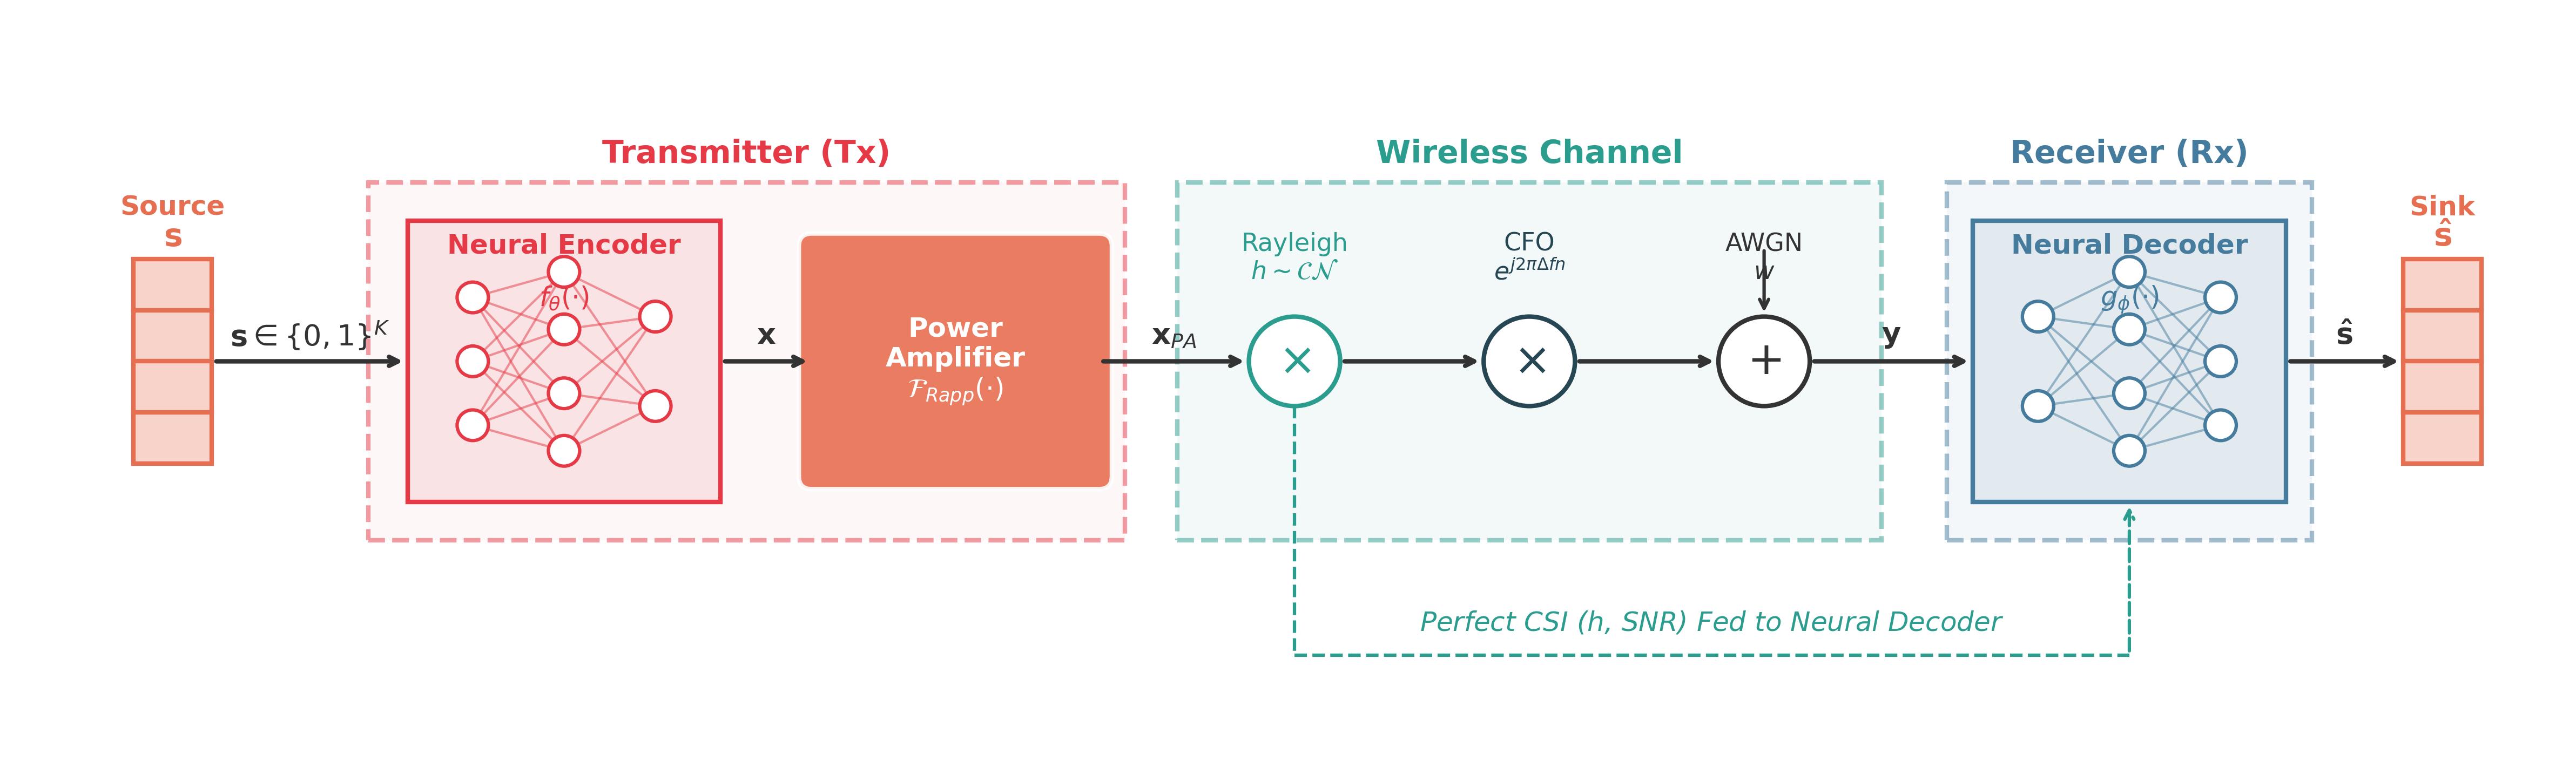
\includegraphics[width=0.78\linewidth]{assets/system_diagram.png}\\[-1mm]
  {\scriptsize Chuỗi suy hao được đưa vào lớp kênh khả vi để huấn luyện end-to-end.}
\end{frame}

% 5
\begin{frame}{Cơ Sở AutoEncoder Cho Lớp Vật Lý}
  \begin{columns}[T,onlytextwidth]
    \begin{column}{0.45\textwidth}
      \centering
      \img{0.80}{autoencoder.png}
    \end{column}
    \begin{column}{0.53\textwidth}
      \begin{block}{Diễn giải truyền thông}
      \begin{itemize}
        \item Encoder: ánh xạ bit/ký hiệu sang điểm IQ.
        \item Channel layer: mô phỏng suy hao vật lý.
        \item Decoder: ước lượng hậu nghiệm ký hiệu hoặc bit.
      \end{itemize}
      \end{block}
      \begin{equation*}
      \theta^\star = \arg\min_\theta \mathbb{E}\big[\mathcal{L}(s,\hat{s}_\theta(y))\big].
      \end{equation*}
      \vspace{1mm}
      {\small\textbf{\color{MtaBlue}Ý nghĩa.} Điều chế và giải điều chế được tối ưu đồng thời theo tiêu chuẩn lỗi trên chính phân bố suy hao của kênh.}
    \end{column}
  \end{columns}
\end{frame}

% 6
\begin{frame}{Kiến Trúc 1: AE Đơn Ký Hiệu Kháng PA}
  \begin{columns}[T,onlytextwidth]
    \begin{column}{0.52\textwidth}
      \begin{block}{Luồng xử lý}
      One-hot $s\in\{0,1\}^{16}$ $\rightarrow$ MLP Encoder $\rightarrow$ IQ $\rightarrow$ PA + Rayleigh + AWGN $\rightarrow$ MLP Decoder + Softmax.
      \end{block}
      \begin{equation*}
      x_{\text{norm}}=\frac{x_{\text{raw}}}{\sqrt{\mathbb{E}\|x_{\text{raw}}\|^2+\epsilon}}.
      \end{equation*}
      \begin{equation*}
      \mathcal{L}= \mathcal{L}_{CE}
      +\lambda_P \mathbb{E}\left[\max(\|x\|-\gamma A_{sat},0)^2\right].
      \end{equation*}
    \end{column}
    \begin{column}{0.46\textwidth}
      \centering
      \img{0.88}{pa_curve.png}\\[-1mm]
      {\scriptsize Hàm phạt công suất ép chòm sao tránh vùng bão hòa PA.}
    \end{column}
  \end{columns}
\end{frame}

% 7
\begin{frame}{Học Hình Học Chòm Sao Dưới Méo PA}
  \begin{columns}[T,onlytextwidth]
    \begin{column}{0.32\textwidth}
      \centering
      \img{0.86}{qam16.png}
      {\scriptsize 16-QAM trước PA}
    \end{column}
    \begin{column}{0.32\textwidth}
      \centering
      \img{0.86}{qam16_after_pa.png}
      {\scriptsize 16-QAM sau PA}
    \end{column}
    \begin{column}{0.32\textwidth}
      \centering
      \img{0.86}{ae_constellation.png}
      {\scriptsize Chòm sao AE học được}
    \end{column}
  \end{columns}
  \vspace{1mm}
  \begin{block}{Nhận xét kỹ thuật}
  AE không giữ lưới chữ nhật đều như 16-QAM; các điểm được phân bố lại để tránh vùng nén biên độ và tăng khoảng cách hiệu dụng sau PA.
  \end{block}
\end{frame}

% 8
\begin{frame}{Kết Quả 1: Rayleigh + PA + AWGN}
  \begin{columns}[T,onlytextwidth]
    \begin{column}{0.60\textwidth}
      \centering
      \img{0.98}{ber_scenario1.png}
    \end{column}
    \begin{column}{0.38\textwidth}
      \begin{block}{Kết quả chính}
      \begin{itemize}
        \item Từ khoảng SNR $\geq 14$ dB, AE tách khỏi 16-QAM + ZF.
        \item Tại BER $10^{-2}$: lợi SNR khoảng \gain{3--4 dB}.
        \item Tại 34 dB: BER AE $\approx 6\times10^{-4}$, thấp hơn khoảng \gain{4 lần}.
      \end{itemize}
      \end{block}
      \smallref{Điểm mạnh xuất hiện rõ khi nhiễu cộng không còn là suy hao chi phối.}
    \end{column}
  \end{columns}
\end{frame}

% 9
\begin{frame}{Kiến Trúc 2: AE Nhiều Ký Hiệu Cho Bù CFO Mù}
  \begin{columns}[T,onlytextwidth]
    \begin{column}{0.48\textwidth}
      \centering
      \img{0.90}{multisymbol_ae.png}
    \end{column}
    \begin{column}{0.50\textwidth}
      \begin{block}{Ý tưởng}
      Encoder dùng Time-Distributed MLP để tạo chuỗi $L$ ký hiệu; Decoder quan sát cả block nhận được để suy ra xu thế quay pha.
      \end{block}
      \begin{equation*}
      y_{\text{cfo}}[n]=x_{\text{pa}}[n]e^{j2\pi\Delta f T_s n}+w[n].
      \end{equation*}
      \begin{itemize}
        \item $\Delta f T_s$ thay đổi trong huấn luyện nhưng không cấp trực tiếp cho Decoder.
        \item Decoder học bù CFO mù, không dùng PLL/pilot.
      \end{itemize}
    \end{column}
  \end{columns}
\end{frame}

% 10
\begin{frame}{CFO: Từ Méo Quỹ Đạo Đến Lợi Ích Học Chuỗi}
  \begin{columns}[T,onlytextwidth]
    \begin{column}{0.40\textwidth}
      \centering
      \img{0.92}{cfo_effect.png}
      \vspace{1mm}
      {\scriptsize CFO tạo quỹ đạo quay pha tích lũy theo chỉ số ký hiệu.}
    \end{column}
    \begin{column}{0.58\textwidth}
      \begin{block}{Cơ chế học}
      AE không ước lượng CFO bằng công thức tường minh; mạng học ánh xạ phi tuyến từ hình dạng quỹ đạo nhận được về chuỗi ký hiệu ban đầu.
      \end{block}
      \begin{itemize}
        \item Quyết định theo block làm giảm nhạy với nhiễu tức thời.
        \item Tín hiệu tương quan theo thời gian trở thành nguồn thông tin để bù pha.
      \end{itemize}
      \begin{equation*}
      \hat{\mathbf{s}}=\arg\max_{\mathbf{s}}p_\theta(\mathbf{s}\mid \mathbf{y}_{1:L},\text{SNR}).
      \end{equation*}
    \end{column}
  \end{columns}
\end{frame}

% 11
\begin{frame}{Kết Quả 2: Bù CFO Mù Trên Kênh Tổng Hợp}
  \begin{columns}[T,onlytextwidth]
    \begin{column}{0.50\textwidth}
      \centering
      \img{0.88}{ber_cfo_0005.png}
      {\scriptsize $\Delta fT_s=0.005$}
    \end{column}
    \begin{column}{0.50\textwidth}
      \centering
      \img{0.88}{ber_cfo_001.png}
      {\scriptsize $\Delta fT_s=0.01$}
    \end{column}
  \end{columns}
  \vspace{0.5mm}
  \begin{block}{Kết luận từ mô phỏng}
  Khi CFO tăng, 16-QAM + ZF xuất hiện error floor; AE vẫn giảm BER theo SNR và đạt lợi khoảng \gain{5--8 dB} tại BER $10^{-2}$.
  \end{block}
\end{frame}

% 12
\begin{frame}{Kiến Trúc 3: Neural FEC Kết Hợp Điều Chế Và Sửa Lỗi}
  \begin{columns}[T,onlytextwidth]
    \begin{column}{0.46\textwidth}
      \begin{block}{Khác biệt so với điều chế cổ điển}
      Thay vì ánh xạ $k$ bit vào một ký hiệu duy nhất, Encoder ánh xạ $k$ bit vào $N$ điểm IQ, tạo dư thừa trong miền Euclid.
      \end{block}
      \begin{equation*}
      R=\frac{k}{2N},\qquad
      \hat{b}_i=\sigma(f_{\theta,i}(\mathbf{y}_{1:N})).
      \end{equation*}
      \begin{itemize}
        \item Đầu vào: vector bit thô, không cần one-hot.
        \item Đầu ra: xác suất từng bit bằng Sigmoid.
      \end{itemize}
    \end{column}
    \begin{column}{0.52\textwidth}
      \centering
      \img{0.98}{ber_neural_fec.png}
      {\scriptsize AE $4\rightarrow6$ đạt BER $<10^{-4}$ ở khoảng 8 dB trong kịch bản đánh giá.}
    \end{column}
  \end{columns}
\end{frame}

% 13
\begin{frame}{Huấn Luyện: Curriculum Learning Và Hàm Mất Mát Có Ràng Buộc}
  \begin{columns}[T,onlytextwidth]
    \begin{column}{0.52\textwidth}
      \begin{block}{Curriculum learning}
      Huấn luyện đi từ kênh dễ đến kênh khó: SNR cao $\rightarrow$ dải SNR rộng; CFO nhỏ $\rightarrow$ CFO lớn; sau cùng tinh chỉnh với learning rate thấp.
      \end{block}
      \begin{equation*}
      \mathcal{L}_{2}= \mathcal{L}_{CE}
      +\lambda_P P_{\text{sat}}
      +\lambda_D\max(d_{\text{target}}^2-d_{\min}^2,0).
      \end{equation*}
    \end{column}
    \begin{column}{0.46\textwidth}
      \begin{table}
      \scriptsize
      \begin{tabularx}{\linewidth}{lccc}
      \toprule
      Tham số & Sc.1 & Sc.2 & Sc.3\\
      \midrule
      Số pha & 3 & 4 & 3\\
      Batch & 4096 & 4096 & 4096\\
      Max CFO & 0 & 0.03 & 0.03\\
      $A_{sat},p$ & 1.2,3 & 1.2,3 & 1.2,3\\
      Optimizer & Adam & Adam & Adam\\
      \bottomrule
      \end{tabularx}
      \end{table}
      \begin{itemize}
        \item Gradient clipping $\|\nabla\|\leq1$.
        \item BatchNorm, dropout nhẹ, early stopping.
      \end{itemize}
    \end{column}
  \end{columns}
\end{frame}

% 14
\begin{frame}{Khả Năng Tích Hợp: Soft LLR Và BIBCM-ID/LDPC}
  \begin{columns}[T,onlytextwidth]
    \begin{column}{0.48\textwidth}
      \begin{equation*}
      L(b_i)=\ln
      \frac{\sum_{m:b_i(m)=1}P(s_m\mid\mathbf{y})}
           {\sum_{m:b_i(m)=0}P(s_m\mid\mathbf{y})}.
      \end{equation*}
      \begin{block}{Điểm quan trọng}
      Softmax của Decoder không chỉ cho hard decision, mà còn cung cấp xác suất hậu nghiệm để trích LLR mềm cho bộ giải mã Turbo/LDPC.
      \end{block}
    \end{column}
    \begin{column}{0.50\textwidth}
      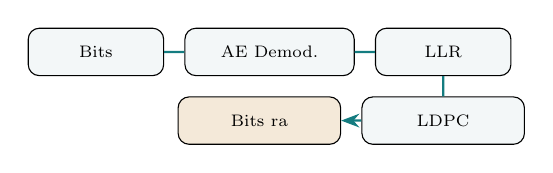
\begin{tikzpicture}[font=\scriptsize, node distance=3mm, scale=0.86, transform shape]
        \node[draw,rounded corners,fill=MtaSoft,minimum width=20mm,minimum height=7mm] (bits) {Bits};
        \node[draw,rounded corners,fill=MtaSoft,right=of bits,minimum width=25mm,minimum height=7mm] (ae) {AE Demod.};
        \node[draw,rounded corners,fill=MtaSoft,right=of ae,minimum width=20mm,minimum height=7mm] (llr) {LLR};
        \node[draw,rounded corners,fill=MtaSoft,below=of llr,minimum width=24mm,minimum height=7mm] (ldpc) {LDPC};
        \node[draw,rounded corners,fill=MtaGold!20,left=of ldpc,minimum width=24mm,minimum height=7mm] (out) {Bits ra};
        \draw[-{Stealth},thick,MtaTeal] (bits)--(ae)--(llr)--(ldpc)--(out);
      \end{tikzpicture}
      \vspace{3mm}
      \begin{itemize}
        \item Phù hợp với tư duy BIBCM-ID: trao đổi thông tin mềm giữa Demodulation và giải mã kênh.
        \item AE có thể được xem như bộ Demodulation thông minh trong chuỗi thu hiện hữu.
      \end{itemize}
    \end{column}
  \end{columns}
\end{frame}

% 15
\begin{frame}{Kết Luận Và Hướng Phát Triển}
  \begin{columns}[T,onlytextwidth]
    \begin{column}{0.47\textwidth}
      \begin{block}{Kết luận chính}
      \begin{itemize}
        \item AE học chòm sao kháng PA, đạt lợi SNR \gain{3--4 dB}.
        \item AE nhiều ký hiệu bù CFO mù, đạt lợi \gain{5--8 dB} so với 16-QAM + ZF trong kịch bản CFO.
        \item Neural FEC cho thấy khả năng hợp nhất điều chế và sửa lỗi trong một ánh xạ học được.
      \end{itemize}
      \end{block}
    \end{column}
    \hfill
    \begin{column}{0.47\textwidth}
      \begin{block}{Giới hạn và hướng tiếp theo}
      \begin{itemize}
        \item Cần kiểm chứng trên OFDM và kênh chọn lọc tần số.
        \item Cần đánh giá độ phức tạp, lượng tử hóa và SDR.
        \item Cần mở rộng giao diện LLR để tích hợp chặt với LDPC/BIBCM-ID.
      \end{itemize}
      \end{block}
      \smallref{Tài liệu nền: Proakis \& Salehi 2008; O'Shea \& Hoydis 2017; Cammerer et al. 2020; Aoudia \& Hoydis 2022.}
    \end{column}
  \end{columns}
\end{frame}

\end{document}
